\documentclass[12pt]{article}

\usepackage{sbc-template}

\usepackage{graphicx,url}

\usepackage[brazil]{babel}
\usepackage[utf8]{inputenc}
\sloppy

\title{Estudo Piloto: Predição de Churn e Segmentação Preliminar de Clientes em Telecomunicações}

\author{Matheus Eduardo Laurindo do Rego\inst{1}}

\address{Especialização em Ciência de Dados\\
Universidade Tecnológica Federal do Paraná (UTFPR)
  \email{matheusrego@alunos.utfpr.edu.br}
}

\begin{document}

\maketitle

\begin{abstract}
  This pilot study is a first-cut experiment: a stratified sample of 1,000
  customers from IBM Telco Customer Churn is modeled with only the two
  variables that stand out in an initial exploratory analysis (tenure and
  contract type), default hyperparameters and a decision threshold of 0.5.
  Logistic Regression reaches AUC-ROC of 0.787, accuracy of 75.5\% and
  precision of 55.3\% on the hold-out set. The 198 customers flagged as at
  risk (19.8\% of the sample) expose R\$~11.6k of monthly revenue and split
  into two coarse K-Means groups. The results confirm that the problem is
  tractable, but remain well below the project's operational targets and
  motivate a complete pipeline with the full attribute set, feature
  engineering, threshold calibration and finer segmentation.
\end{abstract}

\begin{resumo}
  Este estudo piloto é um primeiro recorte: uma amostra estratificada de
  1.000 clientes da IBM Telco Customer Churn é modelada apenas com as duas
  variáveis que saltam numa exploração inicial (tempo de relacionamento e
  tipo de contrato), hiperparâmetros padrão e limiar de decisão 0,5. A
  Regressão Logística alcança AUC-ROC de 0,787, acurácia de 75,5\% e
  precisão de 55,3\% no teste. Os 198 clientes sinalizados (19,8\% da
  amostra) expõem R\$~11,6 mil de receita mensal e se separam em dois grupos
  grosseiros de K-Means. Os resultados confirmam que o problema é tratável,
  mas ficam claramente abaixo das metas operacionais do projeto e motivam um
  \textit{pipeline} completo com o conjunto inteiro de atributos, engenharia
  de \textit{features}, calibração de limiar e segmentação mais refinada.
\end{resumo}

\section{Introdução}
\label{sec:1}

O custo de adquirir um novo assinante no setor de telecomunicações é
substancialmente maior que o de reter um cliente existente, o que torna a
predição de cancelamento --- o \textit{churn} --- uma alavanca recorrente de
resultado \cite{hadden2007, verbeke2012}. Antes de investir em um
\textit{pipeline} completo de modelagem, entretanto, é prudente executar um
estudo piloto: um experimento reduzido, com desenho deliberadamente simples,
cujo objetivo não é esgotar o problema, mas responder se ele é tratável com os
dados disponíveis e quais decisões metodológicas merecem aprofundamento.

Este documento relata esse primeiro ciclo. A pergunta de pesquisa do piloto
é dupla: (i) um classificador baseline, treinado só com as duas variáveis
que uma exploração inicial já aponta como discriminantes, consegue
identificar clientes em risco com precisão superior à taxa base de
cancelamento? (ii) os clientes sinalizados já se separam em pelo menos dois
perfis interpretáveis, capazes de orientar uma primeira discussão comercial?

O piloto não substitui o estudo completo e não deve ser lido como uma versão
enxuta dele. Ele usa amostra menor, um subconjunto mínimo de atributos,
modelos sem otimização, limiar padrão de 0,5 e agrupamento em apenas dois
segmentos. As metas do projeto --- F-medida e acurácia de 80\%, com núcleos
acionáveis o bastante para a empresa diferenciar o tratamento --- ficam
explicitamente fora do escopo desta etapa. O
que se espera aqui é um diagnóstico de viabilidade e um conjunto de
resultados iniciais que justifiquem, ou não, o investimento no
\textit{pipeline} final.

O texto está organizado da seguinte forma. A Seção~\ref{sec:2} delimita o
escopo e as simplificações. A Seção~\ref{sec:3} descreve a metodologia. A
Seção~\ref{sec:4} apresenta os resultados iniciais. A Seção~\ref{sec:5}
traduz os achados em encaminhamentos para o estudo completo.

\section{Escopo e simplificações do piloto}
\label{sec:2}

Um estudo piloto deve ser menor, mais barato e mais fácil de interpretar do
que o experimento definitivo. As restrições abaixo foram escolhidas para
testar a hipótese de viabilidade sem antecipar as decisões do trabalho
completo --- em especial, sem usar o conjunto inteiro de atributos da base,
que por si só já produz desempenho próximo ao de um modelo tunado.

\begin{itemize}
  \item \textbf{Amostra reduzida.} Em vez dos 7.043 clientes da base, o
        piloto usa 1.000 registros amostrados de forma estratificada pela
        variável alvo, preservando a taxa de cancelamento de 26,5\%.
  \item \textbf{Recorte mínimo de atributos.} Não há engenharia de
        \textit{features} e tampouco se usam as 19 colunas preditoras. O
        modelo vê apenas \texttt{tenure} e \texttt{Contract}, as duas
        variáveis que uma exploração inicial já destaca. Serviços agregados,
        forma de pagamento, fatura e dados demográficos ficam de fora de
        propósito: o piloto testa se o sinal mais óbvio já basta, e não se
        replica o estudo completo com menos linhas.
  \item \textbf{Modelos baseline.} Comparam-se Regressão Logística e Árvore
        de Decisão rasa (\textit{max\_depth} = 3), ambas com hiperparâmetros
        padrão do \textit{scikit-learn} \cite{pedregosa2011}. Não há busca
        bayesiana, ponderação de classes nem \textit{ensemble} de
        \textit{gradient boosting}.
  \item \textbf{Limiar fixo em 0,5.} O ponto de corte não é calibrado. Essa
        escolha é intencional: o piloto deve expor o custo de usar o limiar
        default antes de se investir em calibração.
  \item \textbf{Segmentação grosseira.} Os clientes sinalizados são
        agrupados com K-Means em $K = 2$ \cite{arthur2007}. Não se varre $K$
        nem se compara DBSCAN: o piloto só testa se já há estrutura mínima
        de perfis, sem pretender entregar núcleos prontos para a operação.
\end{itemize}

Essas restrições produzem, por construção, um teto de desempenho inferior ao
do estudo completo. O piloto só é bem-sucedido se, mesmo assim, superar a
seleção aleatória e revelar estrutura mínima nos clientes em risco.

\section{Metodologia}
\label{sec:3}

\subsection{Base e amostra}

A base IBM Telco Customer Churn \cite{ibm2018} contém 7.043 clientes e 21
colunas, com um registro por assinante e sem dimensão temporal. A variável
alvo é binária (\texttt{Churn} = Yes/No), com prevalência de 26,5\% na base
completa. A amostra piloto de 1.000 clientes foi extraída por amostragem
estratificada, com semente fixa, de modo a reproduzir a taxa de
cancelamento da população (26,5\% na amostra).

A divisão treino/teste é 60/40, também estratificada: 600 clientes para
ajuste e 400 para avaliação. A fração de teste é maior que a usual de 20\%
porque o piloto privilegia uma leitura honesta do hold-out em amostra
pequena, e não o máximo de dados para treino. Nenhuma informação do teste
entra no pré-processamento.

\subsection{Pré-processamento e modelos}

A variável numérica \texttt{tenure} é padronizada com
\textit{StandardScaler} ajustado só no treino. A variável categórica
\texttt{Contract} recebe \textit{one-hot encoding}. Os dois classificadores
são:

\begin{itemize}
  \item Regressão Logística, com no máximo 500 iterações;
  \item Árvore de Decisão com profundidade máxima 3, para limitar o
        sobreajuste típico de árvores não podadas em amostras pequenas.
\end{itemize}

A métrica de seleção no piloto é a AUC-ROC, por ser independente do limiar.
Acurácia, precisão, \textit{recall} e F1 da classe churn são reportadas com
o corte de 0,5. A leitura de negócio privilegia a precisão: cada cliente
sinalizado gera um contato comercial, e um falso positivo consome orçamento
de retenção \cite{verbeke2012}.

\subsection{Segmentação preliminar}

O modelo selecionado é aplicado à amostra piloto completa com o mesmo limiar
de 0,5. Os clientes cuja probabilidade estimada ultrapassa o corte formam a
população em risco. Sobre essa subpopulação aplica-se K-Means com $K = 2$,
usando tenure, fatura mensal, tipo de internet e tipo de contrato --- aqui
já se admite um pouco mais de informação do que o classificador viu, apenas
para esboçar perfis. O coeficiente de silhueta \cite{rousseeuw1987} é
registrado como diagnóstico, sem servir de critério de escolha: no piloto,
$K = 2$ é uma decisão de escopo, não de otimização.

\section{Resultados iniciais}
\label{sec:4}

\subsection{Sinais exploratórios na amostra}

Mesmo na amostra de 1.000 clientes, dois padrões clássicos da literatura de
churn já aparecem com clareza (Figura~\ref{fig:eda}). Contratos mensais
concentram a maior parte do cancelamento, enquanto contratos de dois anos
têm taxa residual. O tempo de relacionamento também discrimina: a massa de
cancelamentos se acumula nos primeiros meses. Esses dois sinais foram
exatamente o que definiu o recorte do modelo: o piloto pergunta se eles, sozinhos, já produzem um classificador útil.

\begin{figure}[ht]
\centering
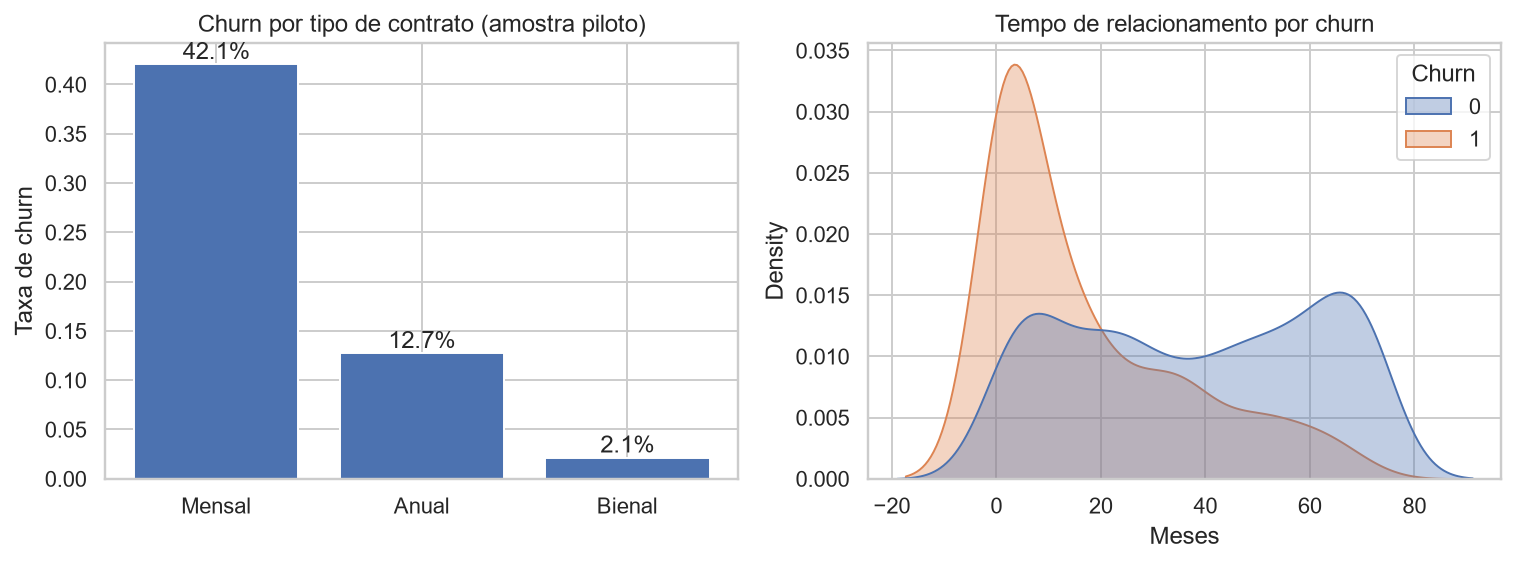
\includegraphics[width=\textwidth]{figuras/eda_piloto.png}
\caption{Sinais exploratórios na amostra piloto: taxa de cancelamento por
tipo de contrato e distribuição do tempo de relacionamento.}
\label{fig:eda}
\end{figure}

\subsection{Desempenho dos baselines}

A Tabela~\ref{tab:modelos} resume as métricas no conjunto de teste de 400
clientes. A Regressão Logística obteve a maior AUC-ROC (0,787) e foi
selecionada. A Árvore de Decisão ficou próxima em acurácia (76,2\% contra
75,5\%), mas com \textit{recall} e F1 ainda mais baixos.

\begin{table}[ht]
\centering
\caption{Desempenho dos modelos baseline no hold-out do piloto (400
amostras, limiar 0,5, apenas \texttt{tenure} e \texttt{Contract}).}
\label{tab:modelos}
\small
\begin{tabular}{|l|c|c|c|c|c|}
\hline
\textbf{Modelo} & \textbf{AUC} & \textbf{Acur.} & \textbf{Prec.} & \textbf{Rec.} & \textbf{F1} \\
\hline
Regressão Logística & 0,787 & 0,755 & 0,553 & 0,396 & 0,462 \\ \hline
Árvore de Decisão   & 0,776 & 0,762 & 0,582 & 0,368 & 0,451 \\
\hline
\end{tabular}
\end{table}

A Figura~\ref{fig:avaliacao} mostra a matriz de confusão, a curva ROC e a
comparação das métricas. Das 106 ocorrências reais de cancelamento no teste,
o modelo logístico identificou 42 (verdadeiros positivos), deixou de
identificar 64 e sinalizou incorretamente 34 clientes que não cancelaram.
A precisão de 55,3\% corresponde a cerca de 2,1 vezes a taxa base de 26,5\%:
pouco mais da metade dos clientes contatados pelo modelo cancelaria de
fato, contra um em cada quatro em uma abordagem sem modelo.

\begin{figure}[ht]
\centering
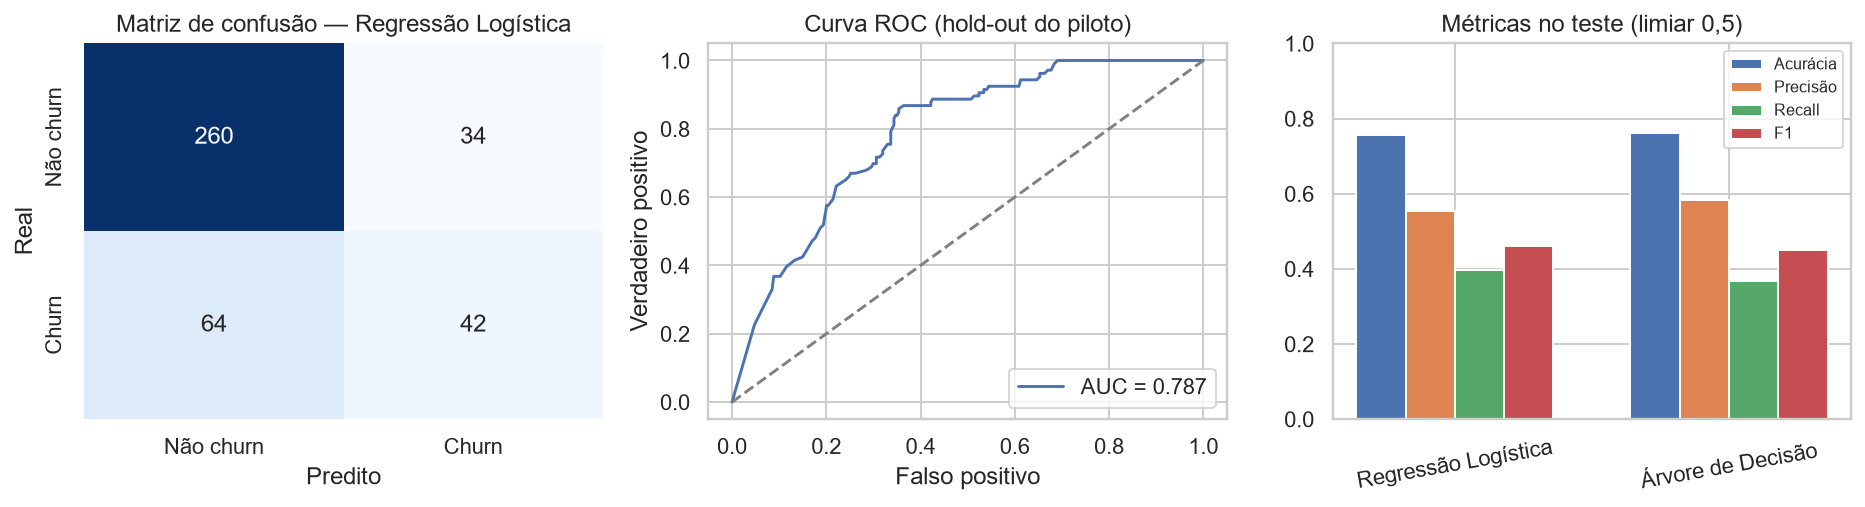
\includegraphics[width=\textwidth]{figuras/avaliacao_piloto.png}
\caption{Avaliação no hold-out do piloto: matriz de confusão e curva ROC da
Regressão Logística, e comparação de métricas entre os dois baselines.}
\label{fig:avaliacao}
\end{figure}

Esses números confirmam um sinal preditivo, mas deixam uma folga evidente em
relação às metas do projeto. A acurácia de 75,5\% mal se distancia da
estratégia ingênua de sempre prever a classe majoritária (73,5\%) e não
atinge os 80\% planejados. A F-medida de 46,2\% e o \textit{recall} de
39,6\% mostram que o recorte de duas variáveis deixa escapar a maior parte
dos cancelamentos. O limiar default de 0,5 e a ausência do restante da
base --- serviços, fatura, forma de pagamento e atributos derivados --- são
as causas mais imediatas dessa folga.

\subsection{População sinalizada e receita exposta}

Aplicada aos 1.000 clientes da amostra, a Regressão Logística sinalizou 198
registros (19,8\%) como em risco. Entre esses clientes, a taxa real de
cancelamento é de 59,6\%, contra 26,5\% na amostra. A soma das faturas
mensais dos sinalizados totaliza R\$~11.590,75. Esse valor não é
comparável à exposição da base completa: trata-se apenas da fatia visível
no recorte piloto, e ainda por cima de uma lista gerada por um modelo que só
enxerga tenure e contrato. Ainda assim, ele já mostra que o problema tem
materialidade financeira e que uma lista sem qualificação de perfil
misturaria clientes de faturas muito distintas.

\subsection{Dois segmentos preliminares}

O K-Means com $K = 2$ separa os 198 sinalizados em dois grupos de mesmo
tamanho, distinguíveis pelo tipo de acesso e pelo patamar de fatura, como
resume a Tabela~\ref{tab:segmentos} e ilustra a Figura~\ref{fig:segmentos}.
O coeficiente de silhueta foi 0,485. Esse valor não deve ser lido como
superior ao de uma segmentação mais refinada sobre a base completa: ele
reflete um corte binário em um espaço pequeno, e não a existência de grupos
naturalmente bem separados para ação comercial.

\begin{table}[ht]
\centering
\caption{Perfil médio dos dois segmentos preliminares de clientes
sinalizados na amostra piloto.}
\label{tab:segmentos}
\small
\begin{tabular}{|l|c|c|}
\hline
\textbf{Característica} & \textbf{Segmento 0} & \textbf{Segmento 1} \\
\hline
Clientes                         & 99      & 99      \\ \hline
Participação nos sinalizados (\%) & 50,0    & 50,0    \\ \hline
Tempo de relacionamento (meses)  & 2,2     & 2,7     \\ \hline
Fatura mensal média (R\$)        & 37,56   & 79,52   \\ \hline
Receita mensal exposta (R\$)     & 3.718,65 & 7.872,10 \\ \hline
Internet predominante            & DSL     & Fibra   \\ \hline
Contrato mensal (\%)             & 100,0   & 100,0   \\ \hline
Taxa real de cancelamento (\%)   & 46,5    & 72,7    \\
\hline
\end{tabular}
\end{table}

\begin{figure}[ht]
\centering
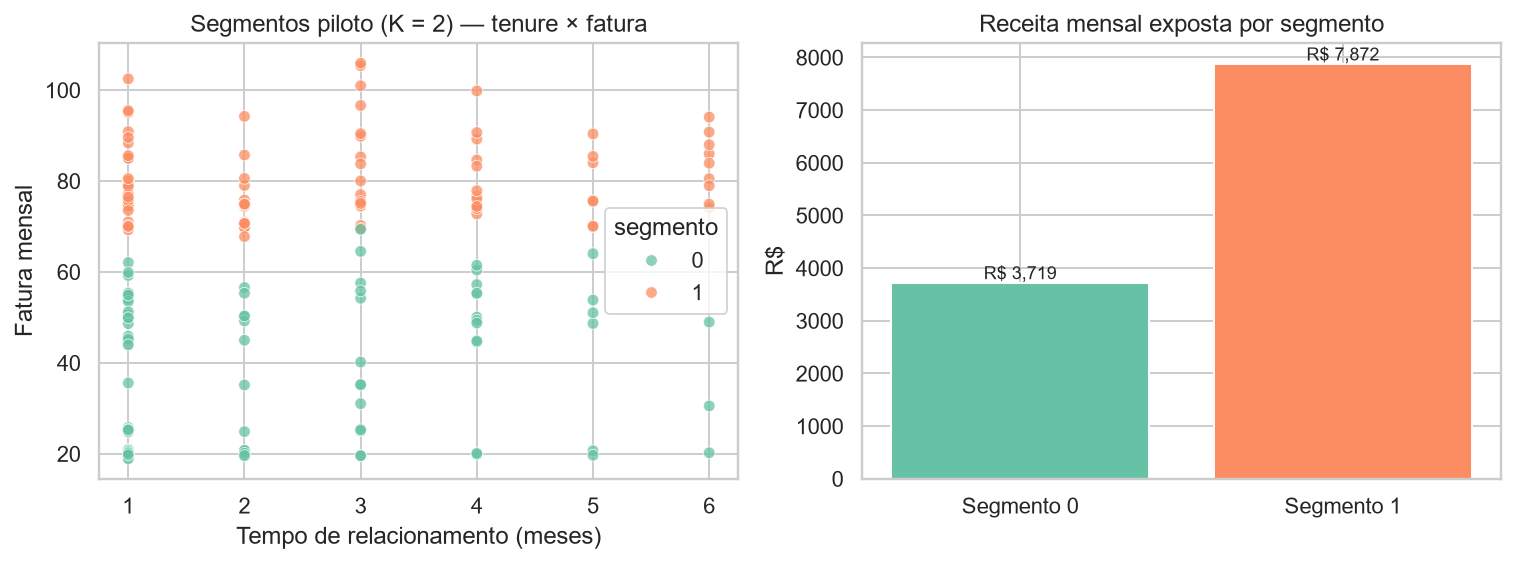
\includegraphics[width=\textwidth]{figuras/segmentos_piloto.png}
\caption{Segmentação preliminar ($K = 2$): dispersão tenure $\times$ fatura
e receita mensal exposta por grupo.}
\label{fig:segmentos}
\end{figure}

A leitura de negócio é útil, porém incompleta. Os dois grupos são clientes
muito recentes e em contrato mensal --- consequência direta do recorte do
classificador. O que os separa é o acesso: o segmento 0, de DSL e fatura
baixa (R\$~37,56), concentra 32\% da receita exposta do piloto e tem taxa
real de cancelamento de 46,5\%; o segmento 1, de fibra e fatura média de
R\$~79,52, concentra 68\% da receita e cancela a 72,7\%. Uma abordagem única
para os 198 nomes trataria da mesma forma um assinante de R\$~38 e um de
R\$~80. Ao mesmo tempo, o corte binário não distingue, dentro da fibra, quem
é cliente recente de quem é veterano de alta fatura --- justamente a
distinção que um $K$ maior e um modelo de risco mais completo precisariam
testar no estudo definitivo.

O piloto também não entrega núcleos prontos para a operação: o corte
binário mistura, na fibra, cliente recente e veterano de alta fatura. Uma
segmentação mais estável, sobre uma lista de risco produzida por um modelo
calibrado, é o que o estudo completo precisa fornecer --- a ação por núcleo
fica com a empresa.

\section{Encaminhamentos para o estudo completo}
\label{sec:5}

Quatro lições do piloto orientam o desenho do trabalho definitivo.

\textbf{Há sinal, mas o recorte mínimo não chega perto das metas.} Superar a
taxa base por um fator de 2,1 valida o uso da IBM Telco como
\textit{proxy}. Não valida a meta de F1 de 80\%, nem sequer a de acurácia,
quando o modelo vê só tenure e contrato. O estudo completo precisa incorporar
o restante dos atributos e testar se variáveis derivadas --- e não apenas
mais um algoritmo --- fecham essa folga.

\textbf{A acurácia sozinha engana.} 75,5\% parece um número aceitável até se
lembrar que prever sempre ``não churn'' já acerta 73,5\%. O estudo completo
deve reportar precisão, \textit{recall} e F1 da classe positiva, e não se
apoiar na acurácia como evidência de sucesso.

\textbf{O limiar default é uma decisão de negócio disfarçada.} Operar em
0,5 misturou 34 falsos positivos e 64 falsos negativos no teste. Uma busca
explícita do ponto de corte, eventualmente dentro da própria otimização de
hiperparâmetros, deve fazer parte do \textit{pipeline} final, privilegiando
precisão em razão do custo do contato \cite{verbeke2012}.

\textbf{Dois segmentos não bastam como núcleos acionáveis.} O corte
fibra versus DSL já mostra que volume e valor não caminham juntos, na linha
dos modelos híbridos de classificação seguida de agrupamento
\cite{ullah2019}. O estudo completo deve restringir o agrupamento aos
clientes sinalizados por um modelo mais completo e testar um $K$ maior,
caracterizando cada perfil em receita exposta --- para que a empresa, e não
o modelo, defina a ação por núcleo.

\section{Conclusão}
\label{sec:6}

Este estudo piloto avaliou a viabilidade de predizer cancelamento e de
esboçar núcleos preliminares sobre uma amostra de 1.000 clientes da base IBM
Telco Customer Churn. Com apenas tempo de relacionamento e tipo de
contrato, modelos baseline e limiar 0,5, a Regressão Logística alcançou
AUC-ROC de 0,787, acurácia de 75,5\% e precisão de 55,3\%. Os 198 clientes
sinalizados expõem R\$~11,6 mil de receita mensal e se separam em dois
grupos grosseiros, um de DSL e baixa fatura e outro de fibra e fatura mais
alta, ambos muito recentes e em contrato mensal.

O experimento cumpre o papel de um piloto: demonstra que o problema é
tratável, quantifica um primeiro ganho sobre a seleção aleatória e aponta
com precisão o que ainda falta --- o conjunto completo de atributos,
engenharia de \textit{features}, calibração de limiar, comparação de
\textit{ensembles} e segmentação mais refinada, com tradução financeira por
perfil. Esses itens constituem o escopo do estudo completo, documentado no
artigo \textit{Predição de Churn e Segmentação Encadeada de Clientes em
Risco no Setor de Telecomunicações}: base integral, 47 atributos derivados,
XGBoost com limiar calibrado e K-Means com $K = 3$ sobre os sinalizados,
gerando núcleos acionáveis --- a saída principal daquele trabalho, sobre a
qual a empresa desenha as próprias campanhas. Os resultados aqui reportados
são iniciais e, por desenho, inferiores aos desse \textit{pipeline}.

\bibliographystyle{sbc}
\bibliography{referencias}

\end{document}
